\newpage % Rozdziały zaczynamy od nowej strony.
\section{Rozwiązanie}
Zadania wizji komputerowej moga zostać podjęta na wiele sposobów. Szczególnie iteresujące są podjeścia do zadania łącznej segmentacji semantycznej i klasyfikacji sceny we wnętrzach. W tym rozdziale przedstawione zostaną wybrane metody, które zostały sprawdzone w ramach analizy problemu. W swoich rozważaniach będę bezpośrednio odnosił się do pytań badawczych postawionych w celu pracy, a więc: 

\begin{itemize}
    \item Jak można zaprojektować model oparty na głębokim uczeniu do wspólnej segmentacji semantycznej i klasyfikacji scen w środowiskach wewnętrznych?
    \item Czy przestrzeń reprezentacji po wytrenowaniu na zadaniu segmentacji semantycznej może być użyta do zadania klasyfikacji sceny?
    \item Jak dobrze proponowany model radzi sobie na dużym zbiorze danych scen wewnętrznych i jak wypada w porównaniu z aktualnymi metodami segmentacji semantycznej i klasyfikacji scen osobno?
    \item Jak proponowany model może być wykorzystany do poprawy wydajności w robotyce mobilnej?
\end{itemize}
Opis rozwiązań problemu zostanie poprzedzony przeglądem rozwiązań. Analiza dotychczasowych pozwoli lepiej ukierunkować badania. Korzystając z doświadczenia innych, będzie można wyrobić sobie intuicję, która pomoże podejmować konkretne decyzje.

\subsection{Przegląd rozwiązań}
Przegląd literatury jest kluczowym aspektem każdej pracy naukowej. W tym rozdziale zostaną przedstawione wyłącznie rozwiązania obejmujące łączną segmentację semantyczną oraz klasyfikację sceny. Szczególny nacisk położony zostanie na architektury głębokich sieci neuronowych z dogłębną analizą przepływu inferencji przez nie.
\vspace{0.5cm}
Niestety przyjetę założenia w pracy nie zostały opisane przez nikogo wczesniej, zgodnie z najlepszą wiedzą autora. Niektóre prace naukowe przedstawiają ten sam problem to jest klasyfikacji i segmentacji łącznie, ale obejmują go w innej domenie danych. Z drugiej artykuły obejmujące środwiska wnętrz są dobrze zdefiniowane, jednak często w swoich rozwiązaniach korzystają z obrazu głębki, który nie zawiera się w zakresie badań tej pracy. Nie mniej wszystkie poniższe artykuły stanowią cenne źródło informacji, które należy mniej lub bardziej dostoswać do rozważanego problemu.

Pierwszym z prezentowanych artykułów jest ,,Describing the Scene as a Whole: Joint Object Detection, Scene Classification and Semantic Segmentation'' autorstwa Yao j. et al (2012)\cite{yao2012describing}. Prezentuje on algorytm, który ówcześnie wyznaczył najlepsze podejście (ang. state-of-the-art (SOTA)). Autorzy wskajzują tutaj, że połączenie rozważanych zadań okazało się owocne nie tylko pod względem jakości, ale również wydajności w kontekście czasowym. Yao J. et al zwracają uwagę na połączenie szeregowe, które niestety propaguje błąd w kolejnych zadaniach, a było dotychczasowo szeroko stosowane. W swojej pracy wykorzysztują podejście równolegle zgodne z rysunkiem \ref{fig:scene-as-a-whole}. Podsumowujac, ,,Describing the Scene as a Whole: Joint Object Detection, Scene Classification and Semantic Segmentation'' nie jest propozycją architektury głębokiej sieci. Wskazuje on na problemy z łączenie, zadań szeregowo, jednocześnie udowadniając, że taka praktyka był ówcześnie stosowana, więc nie można uznawać stosowania połączenia szeregowego jako niedopuszczalnego.

\begin{figure}[ht!]
    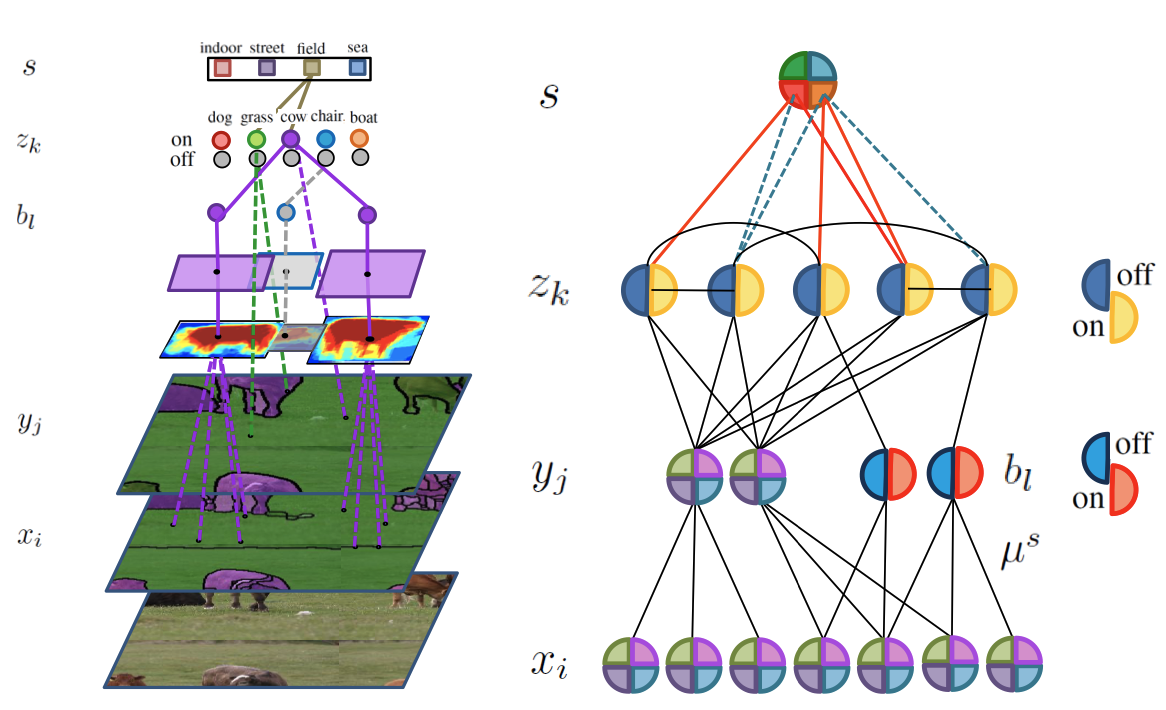
\includegraphics[width=\textwidth]{img/joint-segmentation-and-classification.png}
    \caption{Describing the Scene as a Whole: Joint Object Detection, Scene Classification and Semantic Segmentation (2012) \cite{yao2012describing}.}
    \label{fig:scene-as-a-whole}
\end{figure}

Artykuł ,,Let there be Color!: Joint End-to-end Learning of Global and Local Image Priors for Automatic Image Colorization with Simultaneous Classification 2016 \cite{iizuka2016let}.'' (2016) przedstawia rozwiązanie problemu jednoczesnego klasyfikowania sceny oraz kolorowania zdjęć. Do realizacji zadania kolorowania potrzebna jest sematyczna maska. Wynika z tego, że kolorowanie jest rozszerzeniem segmentacji semantyzcnej. Rozumiejąc towarzyszczące analogie można przejść do analizy rozwiązania. Przedstawiona architektóra (rys.\ref{fig:parrarel-arch}) jest przykładem sieci wielozadaniowej, uzywającej miękkiego dzielenia parametrów, ale tylko i wyłącznie w obrębie pierwszej części sieci. Szczególnie ciekawa jest konkatencja cech wysokiego poziomu (Global Features Network) z cechami średniopoziomowymi (Mid-Level Features Network), która ma miejsce w warstwie fuzji (Fusion layer). Iizuka et al. formułują wniosek oznajmiający o kluczowym znaczeniu tej warstwy w kontekście całego zadania. Wiedza o scenie zdjęcia może dostarczyć informacji wpływających na decyzję, czy na obrazie znajduje się niebo czy trawa. Rozważając sceny wnętrz oczywiste jest, że nie będzie tam takich grup semantycznych. Podsumowując, cechy nauczone na zadaniach klasyfikacj i segmentacji, mogą wzjamniej pozytwnie na siebie wpływać, realizując pozytywny transfer.

\begin{figure}[ht!]
    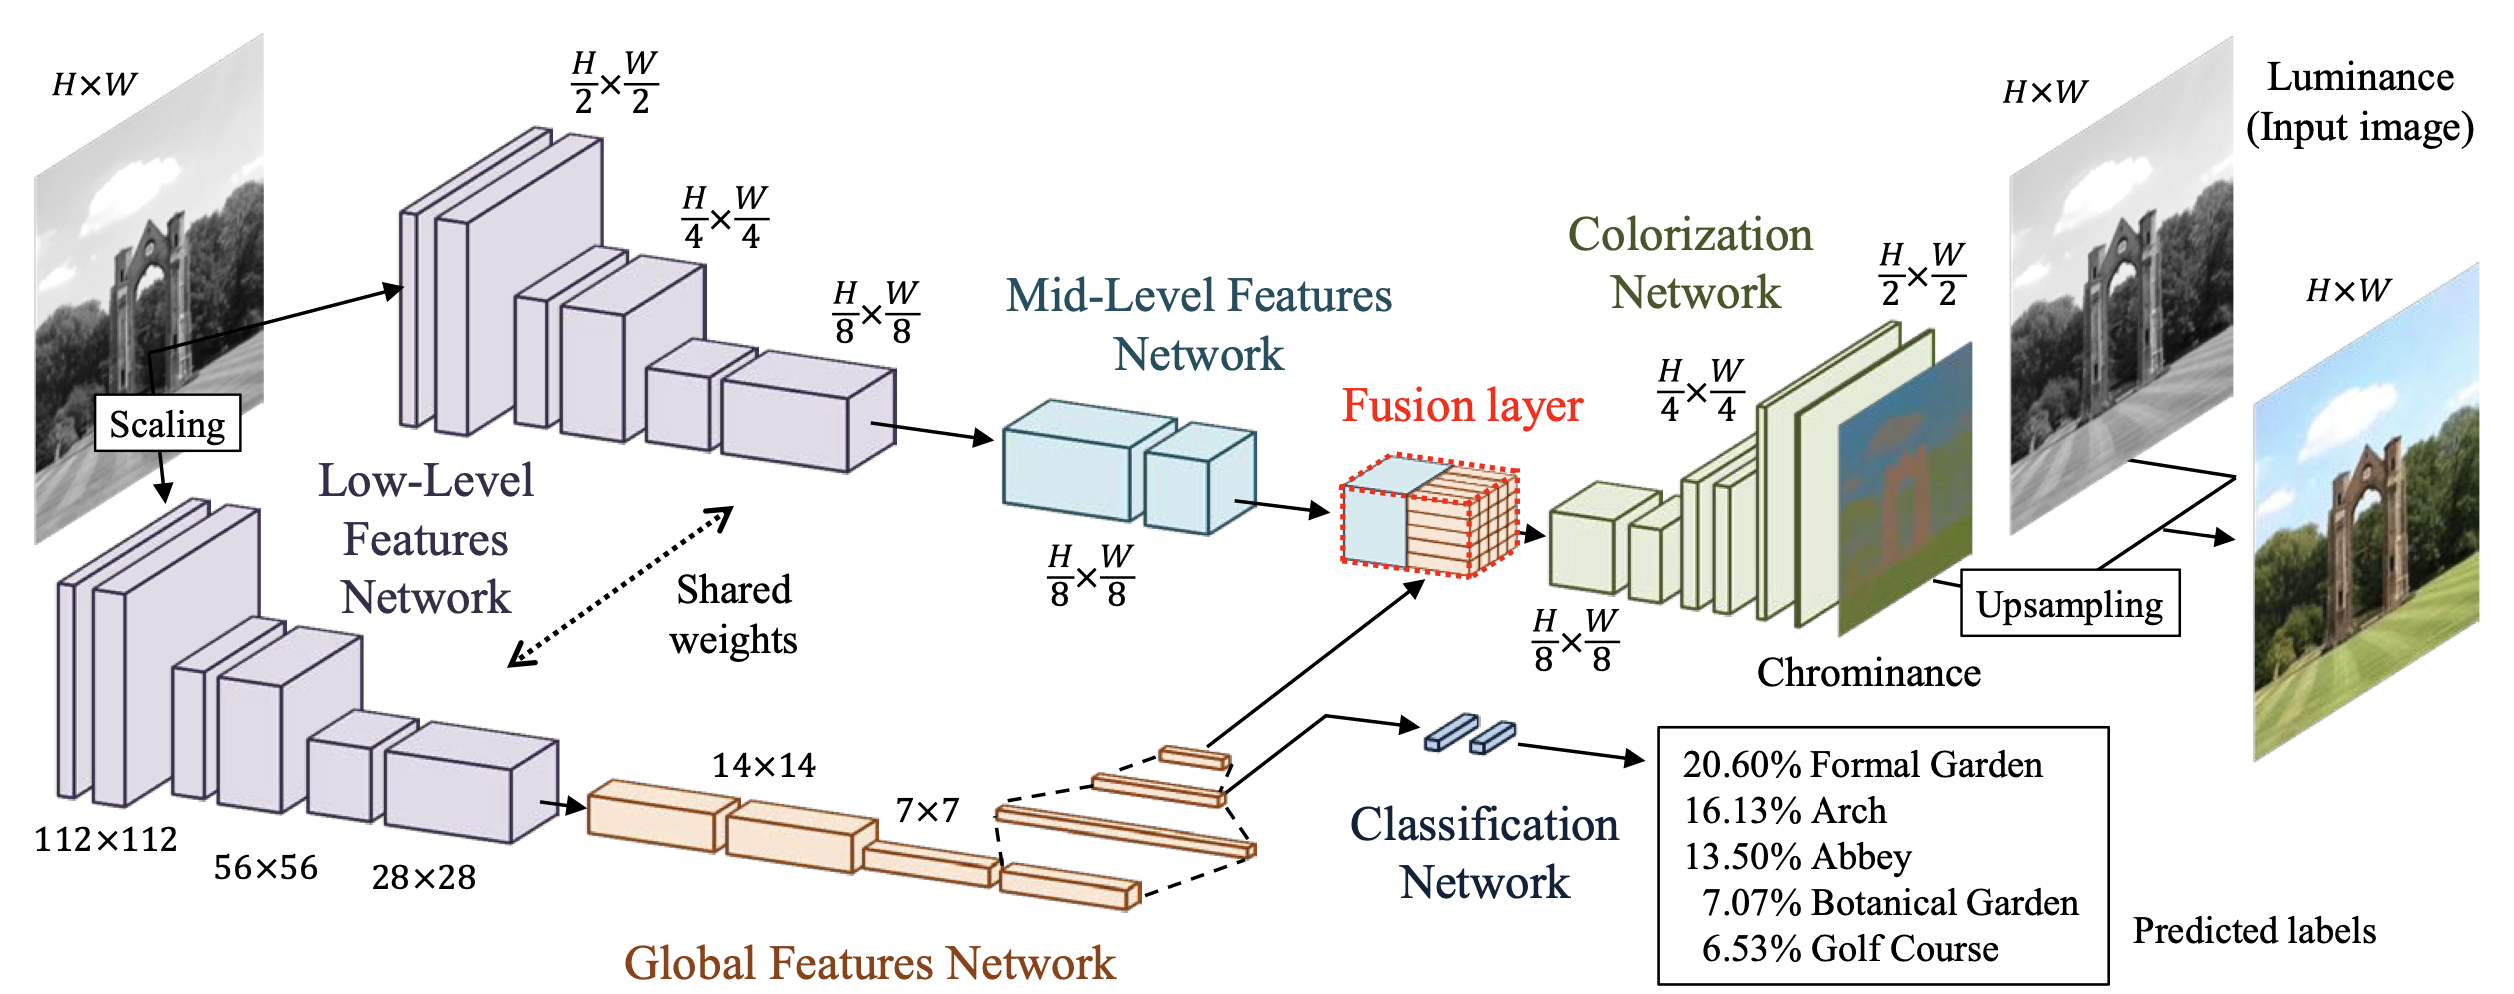
\includegraphics[width=\textwidth]{global-local-features.png}
    \caption{Let there be Color!: Joint End-to-end Learning of Global and Local Image Priors for Automatic Image Colorization with Simultaneous Classification 2016 \cite{iizuka2016let}.}
    \label{fig:parrarel-arch}
\end{figure}

Zastosowanie łącznej segmentacji oraz klasyfikacji tym razem w domenie medycznej przedstawia ,,Y-Net: Joint Segmentation and Classification for Diagnosis of Breast Biopsy Images'' \cite{mehta2018net} (2018). Zadanie te są realizowane przez twarde dzielenie parametrów w kontekście uczenia wielozadaniowego (rys.\ref{fig:y-net}). Architektura jest prostym rozszerzeniem klasycznego U-Netu. Autorzy wskazują, że taki zabieg powodują dużą modulatność, ponieważ do dowolnego modelu segmentacji można podłączyć sieć klasyfikacyjną. Przeprowadzone eksperymenty dla segmentacji udowodniły, że dokładność pozostała na tym samym poziomie. W przypadku klasyfikacji wyniki były wyższe niż dotychczasowe SOTA na tym zbiorze. Jako funkcję straty autorzy użyli sumę entropii skrośnej każdego z zadań. Podsumowując zadanie zadanie segmentacji osiągneło ten sam wysoki wynik co SOTA, a zadanie klasyfikacji ustanowiło nowe SOTA na tym zbiorze uczać się znacznie mniej parametrów.
\begin{figure}[ht!]
    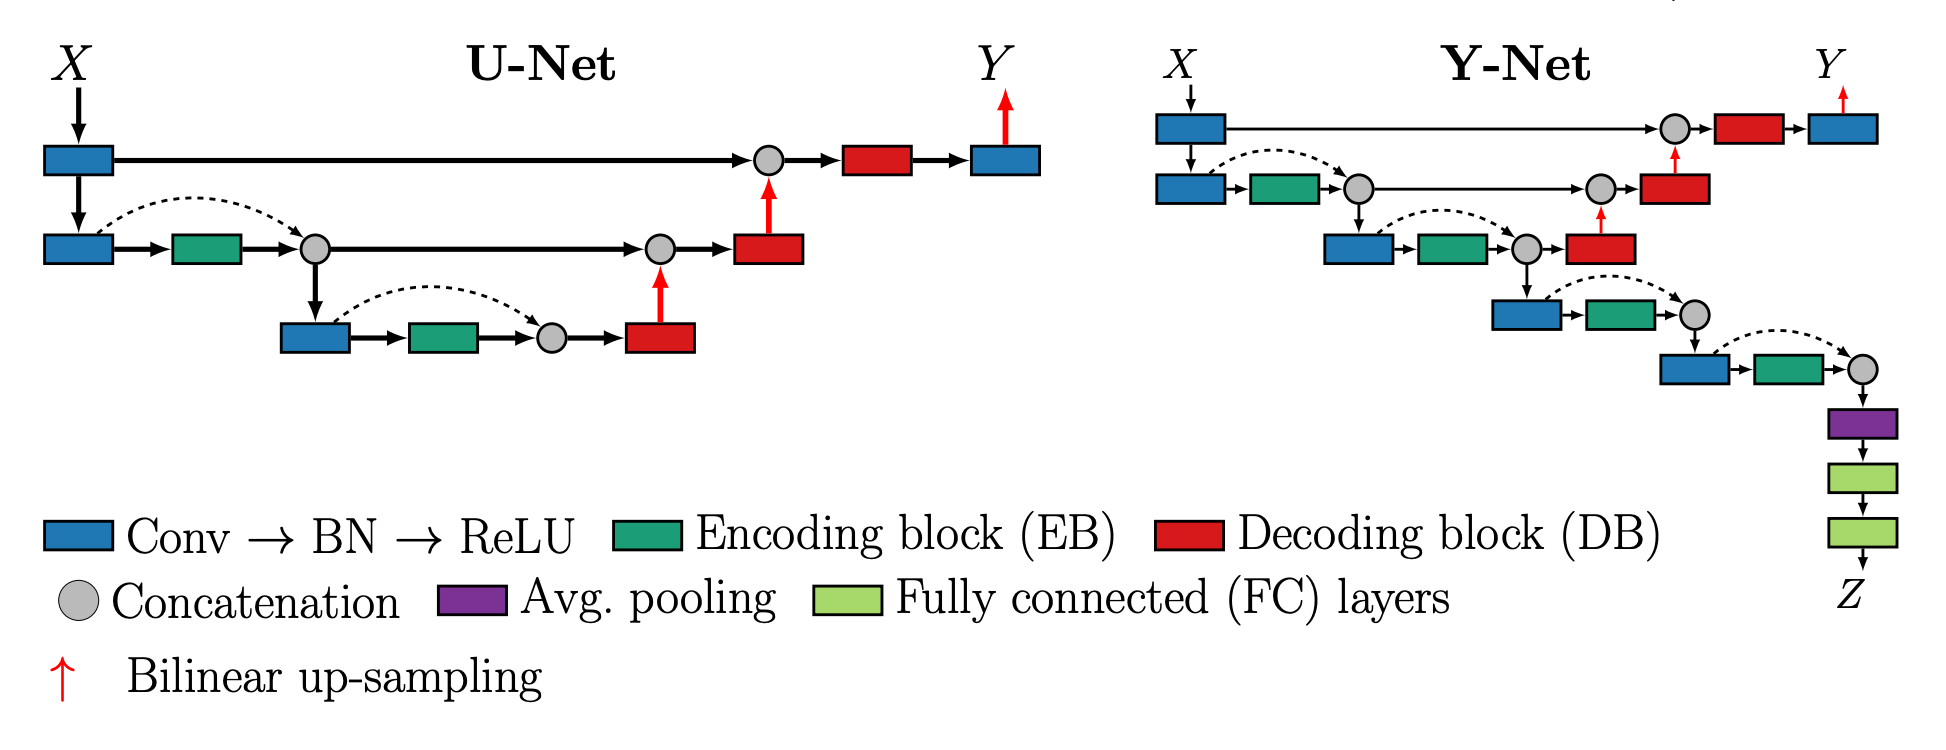
\includegraphics[width=\textwidth]{y-net-new.png}
    \caption{Y-Net: Joint Segmentation and Classification for Diagnosis of Breast Biopsy Images 2018 \cite{mehta2018net}.}
    \label{fig:y-net}
\end{figure}


Najbliższy artykuł tej pracy inżynierskiej jest ,,Efficient Multi-Task RGB-D Scene Analysis for Indoor Environments'' \cite{9892852} (2022), który został opublikowany w czasie tworzenia tej pracy. Przedstawia on jedną głęboką sieć neuronową rozwiązującą następujące zadania: segmentacja semnatyczna oraz segmentacja instacji (łącznie ang. pantopic segmentation), estymacja orientacji instacji oraz klasyfikacja sceny. Rozważaną przez autorów domeną są podbnie jak w przypadku tej pracy sceny wnętrz. Znaczą róznicą poza dodatkowymi zadaniami jest użycie przez zespołu Seichter et al. informacji o głębi. Zgdonie z wnioskami z nieniejszego artykułu przetwarzanie łączne obrazów RGB i głębi jest kluczowe z punktu widzenia jakości predykcji. Każde z zadań zostało na początku trenowane osobno by ustalić punkt odniesienia. Architektura jest przedstawiona na rysunku \ref{fig:emsanet}. Autorzy zdecydowali się na twarde dzielenie parametrów, argumentując całkowitą niezależnością w przypadku chęci wyłączenia jednego zadań z wnioskowania. Trening każdej sieci z osobna był rozważany pod względem wielu backbone'ów ze zróżnicowaniem na uczenie wyłącznie obrazu głebi, obrazu RGB lub RGB-D. Generalnie w przypakdu segmentacji oraz klasyfikacji większy backbone wpływał na polepszenie wyników. Trenując zadania łacznie zdecydowano się na ważoną sumę entropii skrośnej dla zadania segmentacji i klasyfikacji w proporcjach odpowiednio 3:1. Przyjęty krok uczenia, będąć sprawdzonym przez przeszukiwanie liniowe (ang. grid search), jest wyjątkowo duży, bo wynosi 0.02. Autorzy zastosowali zaawansowane techniki dostosowywania kroku czenia w trakcie treningu poprzez użycie planista polityki jednego cyklu (ang. one cycle policy scheduler). Jako optymalizator użyto SGD z momentem oraz drobną regularyzacją. Podsumowujac, zgodnie z prezentowanymi wynikami na wspólnej segmentacji oraz klasyfikacji autorom nie udało się polepszyć działania modelu na segmentacji semantycznej. Z powodzeniem jedank wzrosła dokładność klasyfikacji na zbiorze NYUv2.

\begin{figure}[ht!]
    \centering
    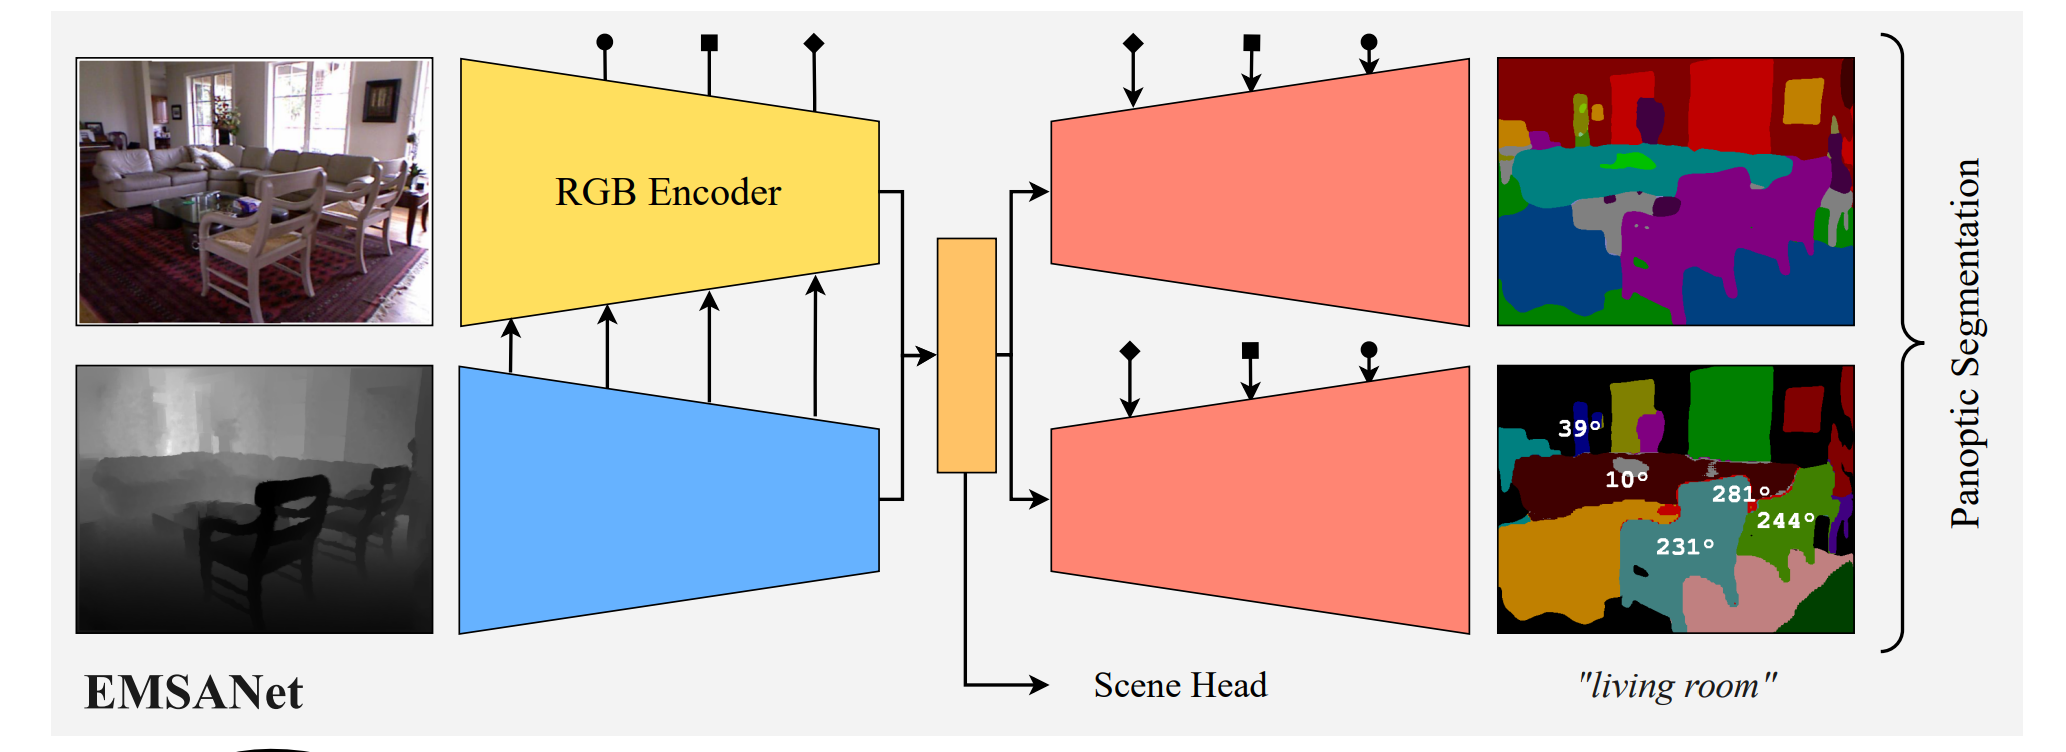
\includegraphics[width=\textwidth]{emsanet.png}
    \caption{Efficient Multi-Task RGB-D Scene Analysis for Indoor Environments \cite{9892852}}
    \label{fig:emsanet}
\end{figure}


\subsection{Rozwiązanie problemu}
W tym rozdziale zostaną przedstawione eksperymenty, które wykonanano w celu zbadania uczenia wielozadniowego segmentacji semantycznej oraz klasyfikacji sceny w domenie pomieszczeń. Pierwszym założeniem jakiego dokonano było wyznaczenie punktu odniesienia. Z punktu widzenia pracy nałatwiej byłoby znaleźć gotowe wyniki segmetnacji oraz klasyfikacji sceny na wybranym zbiorze danych. Niestety żadne z przytaczanych rozwiązań nie odpowiada w pełni zakresowi pracy. Postanowiono stworzyć taki punkt odniesienia samemu przez analogiczne trenowanie sieci segmentacyjnej oraz klasyfikacyjnej osobno.

Posiadając taką wiedzę eksperymentowano dalej z róznymi architekturami uczenia wielozadaniowego. Wybrano uczenie łączne o twardym dzieleniu parametrów. Podejście to ma wiele zalet. \cite{mehta2018net} podkreśla łatwość i wszechstronność implementaji. Wystarczy dołączyć do modelu część klasyfikacyjną. Co więcej wszyscy autorzy (\cite{mehta2018net}, \cite{9892852}) chwalą znacznie mniejszą ilość parametrów sieci co bezpośrednio wpływa na czas treningu oraz wnioskowania. Archtektura sieci przedstawia sie następująco\ref{fig:multitask}. Jest to DeepLabv3 rozszerzony za enkoderem o sieć klasyfikacyjną podbnie jak w artykule \cite{mehta2018net}, gdzie rozszerzono sieć U-Net.
\begin{figure}[ht!]
    \centering
    
\includegraphics[width=0.25\textwidth]{no-image.png}
    \caption{Architektura wielozadaniowej sieci.}
    \label{fig:multitask}
\end{figure}

\subsubsection{Uczenie wielozadaniowe}
Uczenie wielozadaniowe zostało zrealizowane przez architekturę z rysunku \ref{fig:multitask}. Trening polegał na aktualizowaniu wag całego dostępnego modelu zgodnie zgodnie z propagają wsteczną zagregowanej funcji straty $\lambda$. Zaimplementowano ją jako sumę funkcji strat na każdym z zadań, tak jak w przypadku \cite{mehta2018net}. Nie stosowano ważenia zadań \cite{9892852}.
\begin{equation*}
    \lambda = \lambda_{segmentacja} + \lambda_{klasyfikacja}
\end{equation*}

\subsubsection{Wyłącznie klasyfikacja}
W celu określenia punktu odniesienia wytrenowano model zapominając o podsieci do wyznaczania segmetnacji semantycznej. Technicznie skorzystano z modelu wielozadaniowego. Parametry modułów arhitektury takie jak dekoder oraz głowa segmentacyjna zostały zamrożone oraz nie zostały podawane optymalizatorowi w trakcie treningu. Funckja straty $\lambda$ została ograniczona wyłącznie do straty na klasyfikacji poprzez wyzerowanie w kazdym kroku straty na segmentacji

\begin{gather*}
    \lambda = \lambda_{segmentacja} + \lambda_{klasyfikacja} \\
    \lambda_{segmentacja} = 0
\end{gather*}
\subsubsection{Wyłącznie segmentacja}
Analogicznie jak w przypadku klasyfikacji należało określić punkt odniesienia również w przypadku segmentacji. Procedura była taka sama jak w przypadku klasyfikacji. Model wielozadaniowy zamrożono w części klasyfikacyjnej oraz wyłączono zamrożone parametry z optymalizacji. Funkcja straty $\lambda$ została przedstawiona jako
\begin{gather*}
    \lambda = \lambda_{segmentacja} + \lambda_{klasyfikacja} \\
    \lambda_{klasyfikacja} = 0
\end{gather*}
\subsubsection{Finetuning}
Znaną techniką transferu wiedzy jest finetuning. W tym przypadku skorzystano z wytrenowanego enkodera ResNet wytrenowanego na dużej bazie ImageNet. Uczenie przebiegało w dwóch fazach. W pierwszej zamrożono enkoder i starano się osiągnać jak najlepsze rezultaty dysponukąć podsieciami klasyfikacyjną i segmetacyjną. Wynika z tego, że pierwszy etap to ni innego jak uczenie wielozadaniowe ale z wyłączonym enkoderem. Dopiero w drugim etapie odmrażany jest również enkoder. Sytuacja wtedy przypomina wcześniej omawiane uczenie wielozadaniowe. Jendakże, kluczowy jest dobór hiperparametrów. W pierwszym etapie uczenie przebiega z pewny krokiem uczenia. W drugim zaś krok uczenia jest znacznie mniejszy.
\begin{equation*}
    \lambda = \lambda_{segmentacja} + \lambda_{klasyfikacja}
\end{equation*}
\subsubsection{Równoległa klasyfikacja z segmentacji}
Podejście transferu wiedzy można lekko zmodyfikować. Skorzystano z wcześniej przygotowanych wag będących wynikiem wcześniej wspomnianej wyłącznej segmetnacji. Zamrożono enkoder oraz podsieć segmentacyjną oraz wyłączono te parametry z optymalizacji. Następnie dysponując samą podsiecią klasyfikacyjną przeprowadzono trening. Funckja straty była następująca:
\begin{gather*}
    \lambda = \lambda_{segmentacja} + \lambda_{klasyfikacja} \\
    \lambda_{segmentacja} = 0
\end{gather*}
\subsubsection{Szeregowa klasyfikacja z segmentacji}.
Rozwiązaniem odbiegającym od reszty jest przeprowadzenie szeregowej klasyfikacji z segmentacji. Architektura przedstawia się zgodnie z rysunkiem \ref{fig:multitask-parrarel}. W tym eksperymencie sprawdzono jak można skorzystać zgotowych predykcji dotyczących segmentacji. Model aż do głowy segmentacyjnej włącznie został zamkrożony oraz wyłączony z optymalizacji. Zmieniają się tylko wagi części klasyfikacyjnej.

\begin{equation*}
    \lambda = \lambda_{segmentacja} + \lambda_{klasyfikacja}
\end{equation*}







\begin{figure}[ht!]
    \centering
    
\includegraphics[width=0.25\textwidth]{no-image.png}
    \caption{Arhitekrura sieci szeregowej.}
    \label{fig:multitask-parrarel}
\end{figure}

W celu łatwej oraz dokładniej ewaluaji 

W celu lepsze ewaluacji uczenia wielozadaniowego zdecydowano uściślij wszystkie parametry sieci takie jak architekura jest ta sama zeby dało sie porownac nie

nie ma sensu wszystkich scenariusz bo tak

opisać że nie ma sensu porównywać 



Poza uczeniem łącznym zbadano też inne znane techniki uczenia jak finetuning.


% % * multitask Learning
% % * jednozadaniowe
% % * wielozadaniowe
% W celu realizacji zadania zdecydowano się na architekturę (najbliższą Y-Netu) o wspólnym enkoderze i o osobnych głowach, służących do egzekwowania konkretnych zadań (rys. \ref{fig:cep_arch}). Decyzja podyktowana była względnie prostą implementacją rozszerzenia wielu modeli segmentacji semantycznej o dodatkową głowę klasyfikacyjną. Co więcej stwierdzono, że ograniczenie się tylko do jednego backbone'u jest niesłychanie korzystne, gdyż znacząco ogranicza ilość parametrów sieci, co bezpośrednio przekłada się m.in. na czas inferencji. Należy zwrócić uwagę na fakt, iż właściwie zdecydowana większość parametrów znajduje się własnie w enkoderze.

% Mając na uwadze, że symultaniczne uczenie może negatywnie wpływać na jakość uczenia obu zadań, eksperymenty przeprowadzono etapowo. Pierwszym etapem było uczenie jednozadaniowe. Eksperymenty polegały na sprawdzeniu jakości segmentacji oraz klasyfikacji osobno. Wykorzystano do tego tę samą archtekturę, która używana była poźniej w drugim etapie. Mianowicie, mając dwie głowy każdorazowo zamrażano głowę nie biorącą udziału w uczeniu (rys. \ref{fig:arch-scene-seg}). Zapewnia to pewność posiadania tej samej architektury, a w szczególności rzetelne porównanie z etapem uczenia wielozadaniowego.

% Drugim etapem było przeprowadzenie eksperymentów w uczeniu wielozadaniowym (rys. \ref{fig:arch-full}). Funkcja celu zdefiniowana była jako suma wartości funkcji celów dla obu zadań. W wyniku progpagacji wstecznej wagi aktualizowane były zgodnie z zagregowaną stratą.

% Ostatecznie porównano jakość na przesztreni obu etapów.

% \begin{figure}[ht!]
%     \centering
%     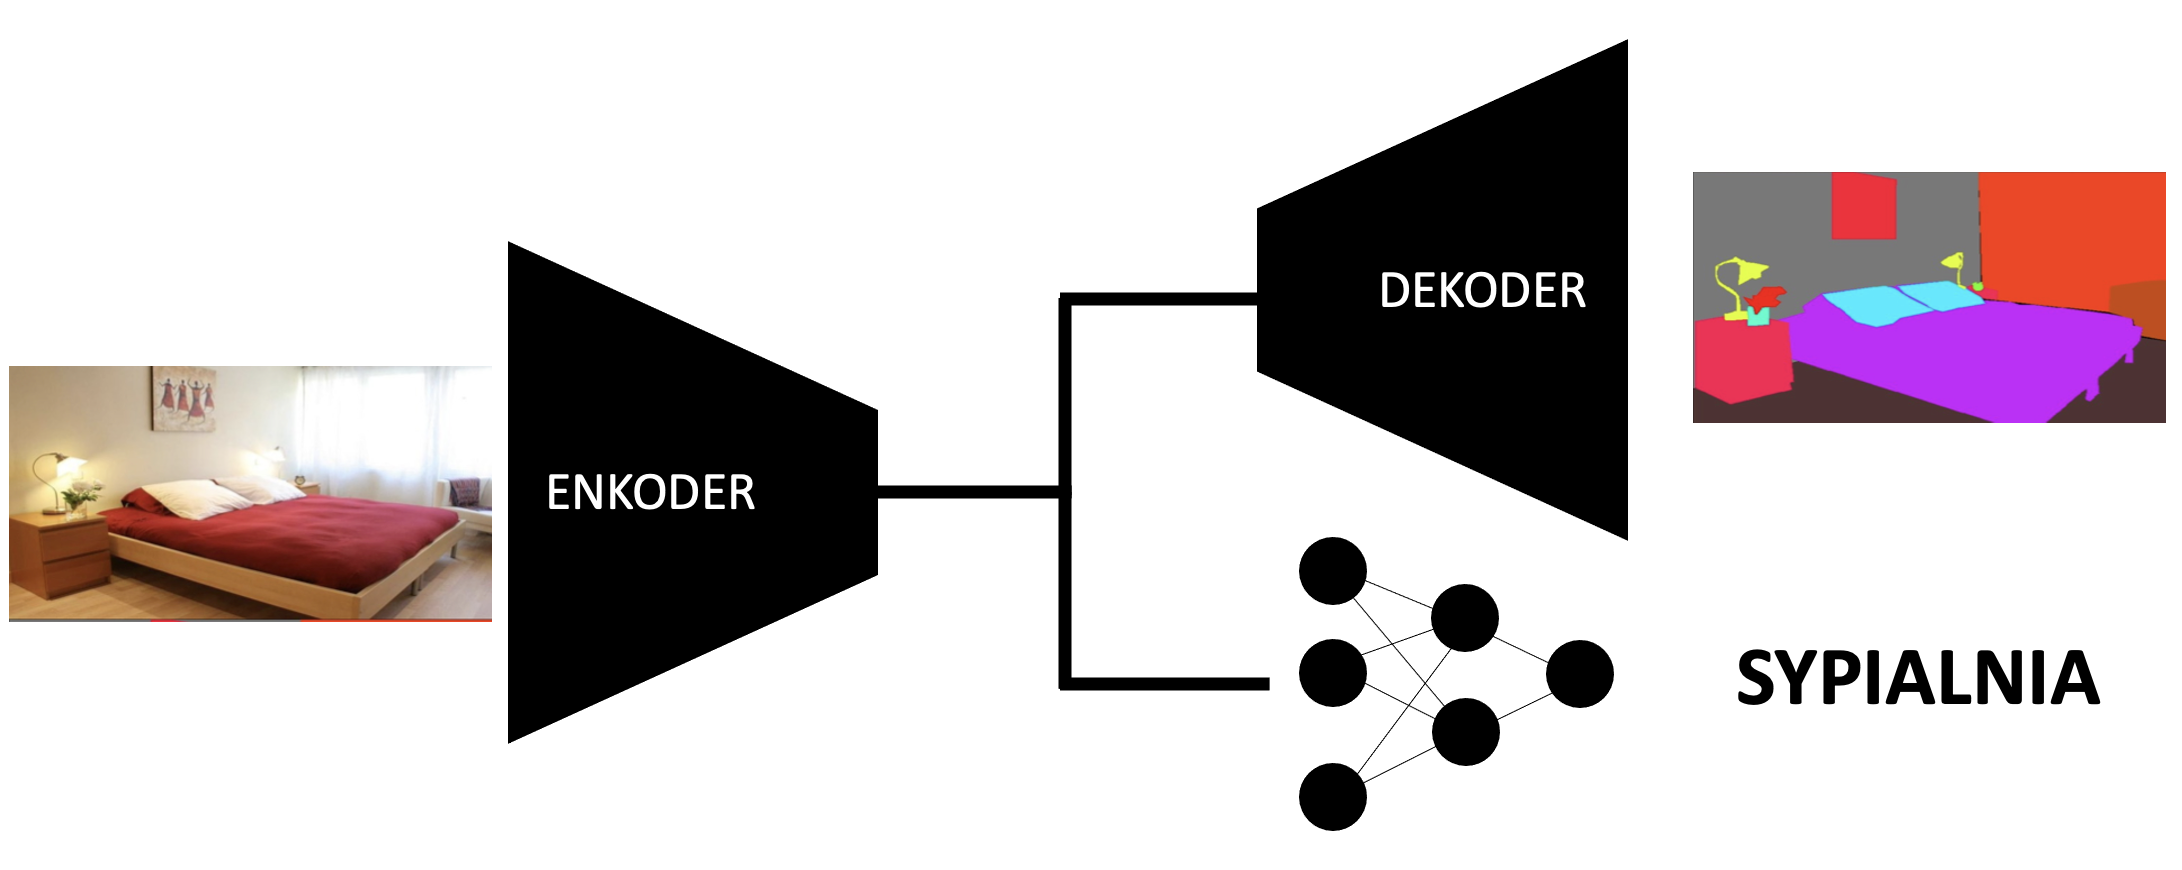
\includegraphics[width=0.75\textwidth]{cep_arch.png}
%     \caption{Architektura sieci zastosowana w pracy inżynierskiej.}
%     \label{fig:cep_arch}
% \end{figure}

% \begin{figure}[ht!]
%     \centering
%     \begin{subfigure}[b]{0.49\textwidth}
%         \centering
%         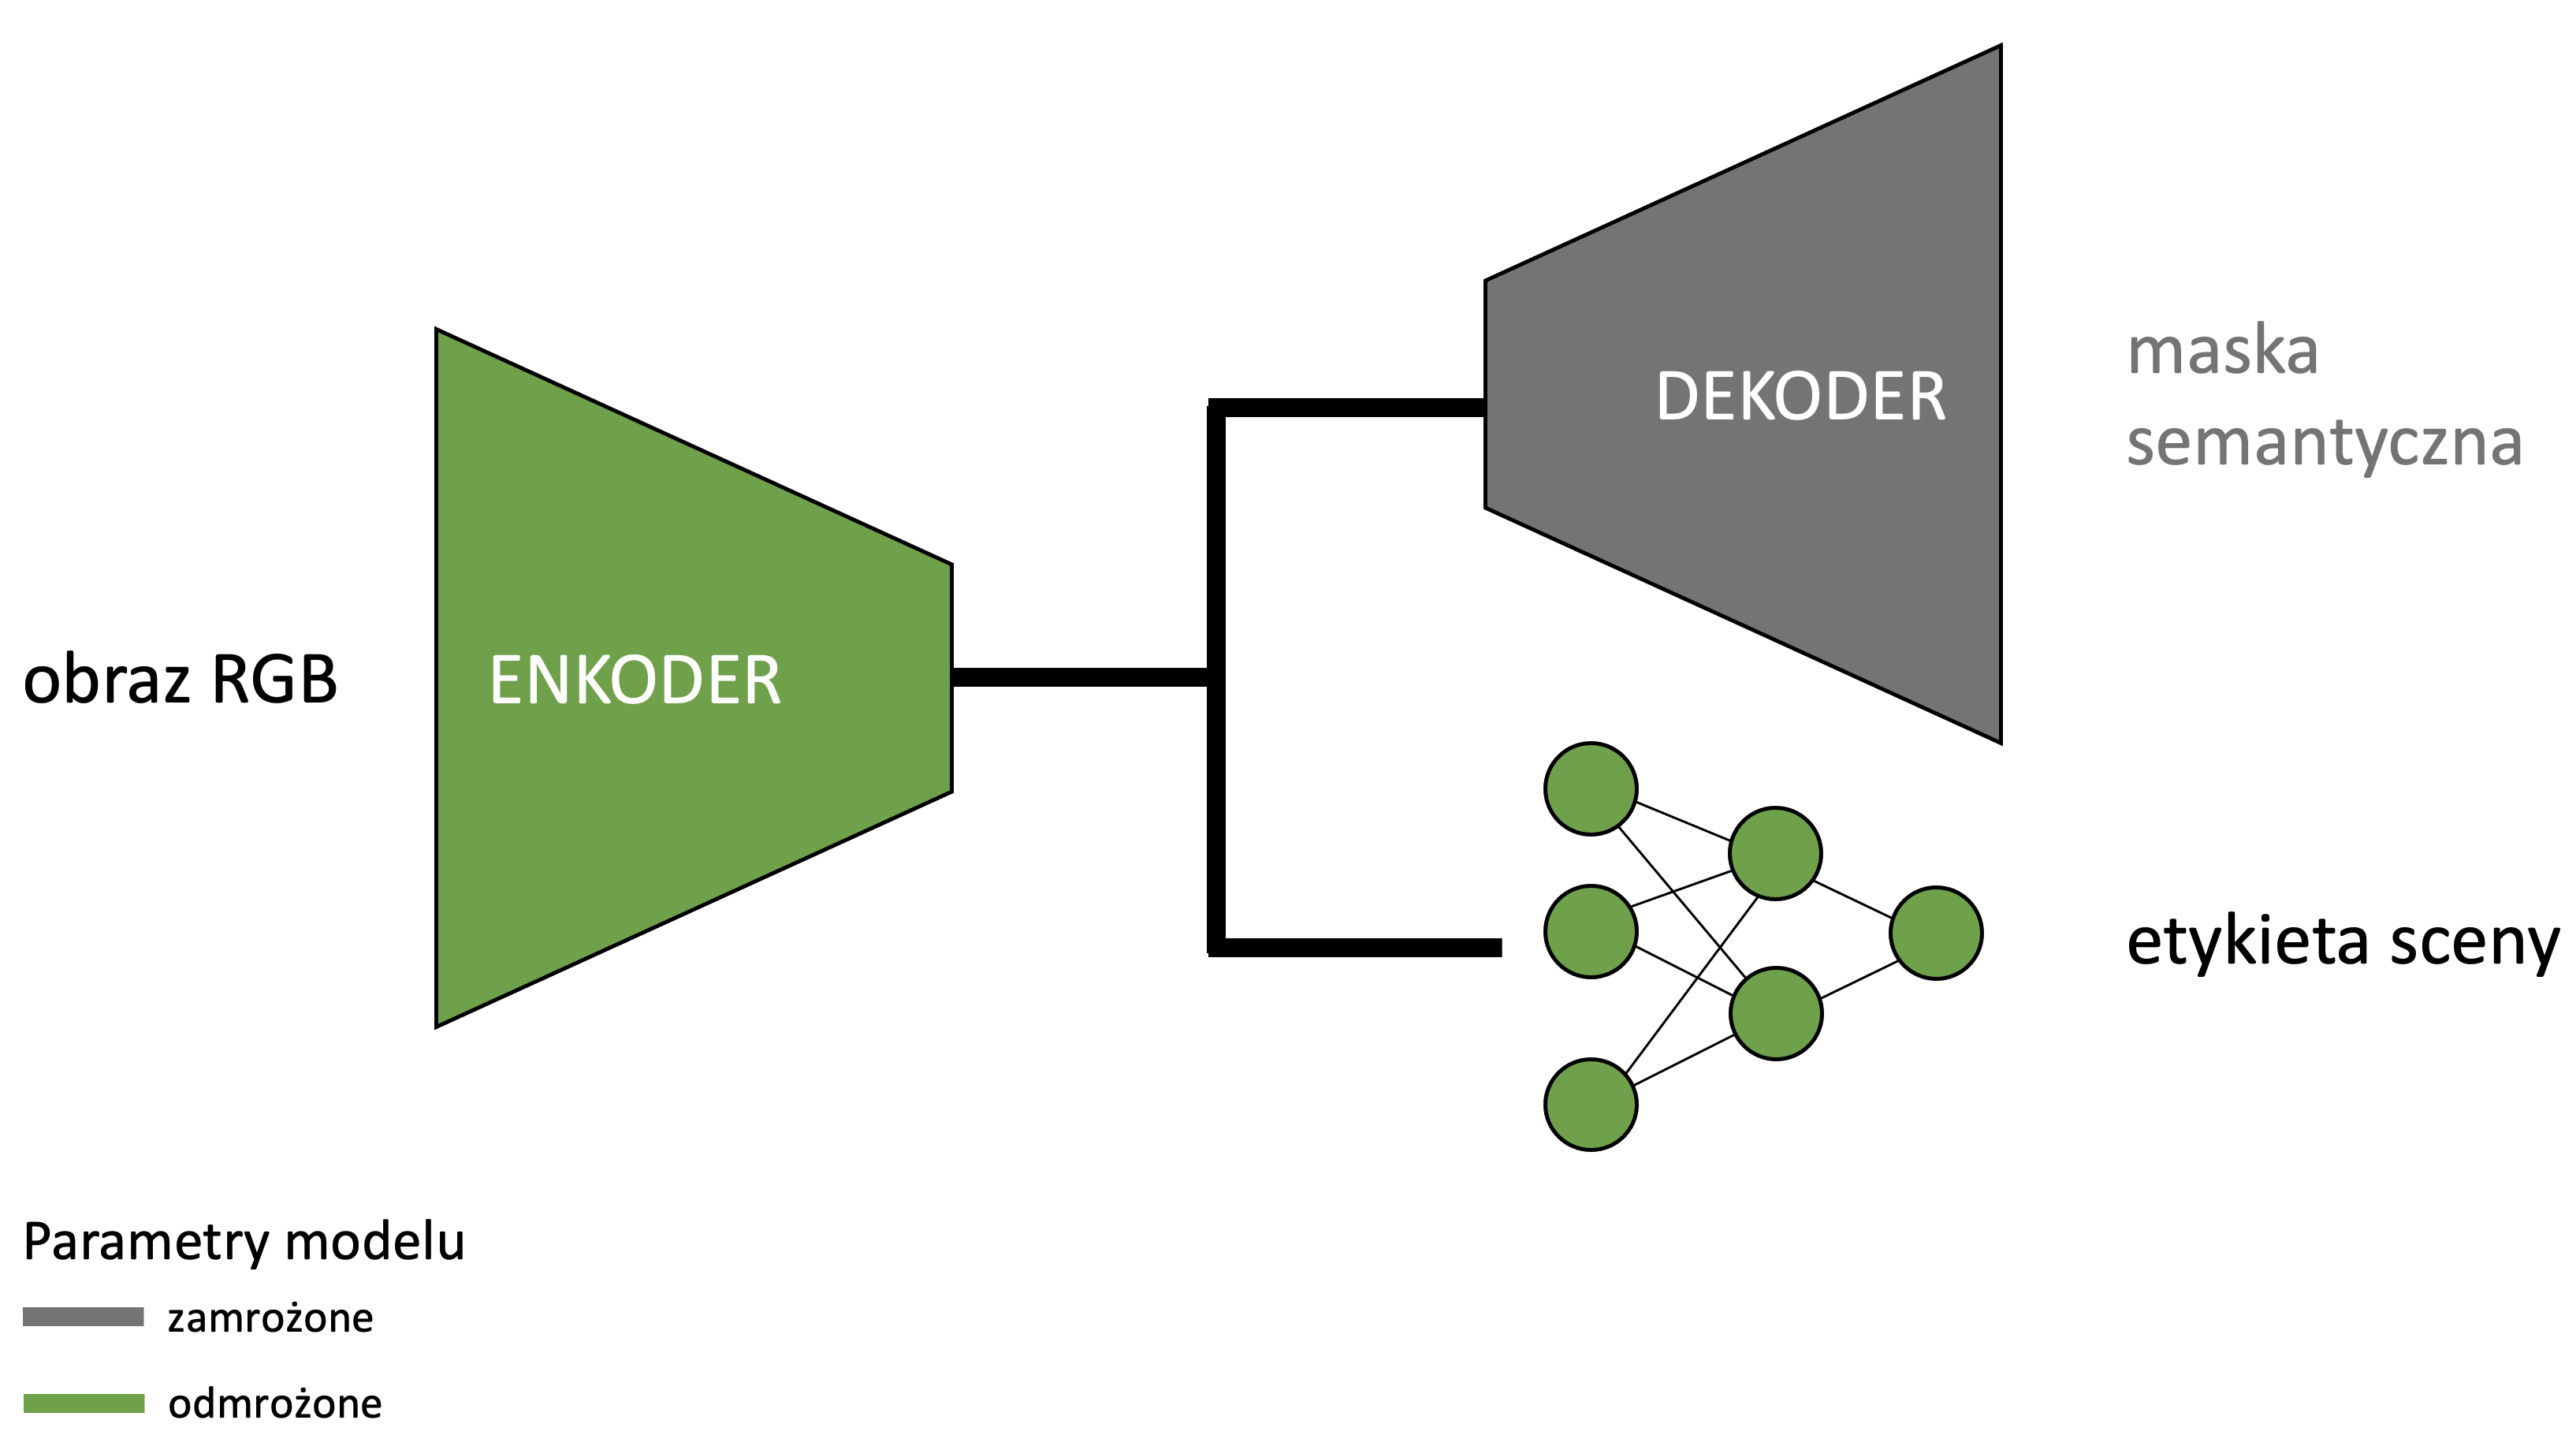
\includegraphics[width=\textwidth]{arch:scene.png}
%         \caption{Architektura sieci wyłącznie w zadaniu klasyfikacji.}
%     \end{subfigure}
%     \hfill
%     \begin{subfigure}[b]{0.49\textwidth}
%         \centering
%         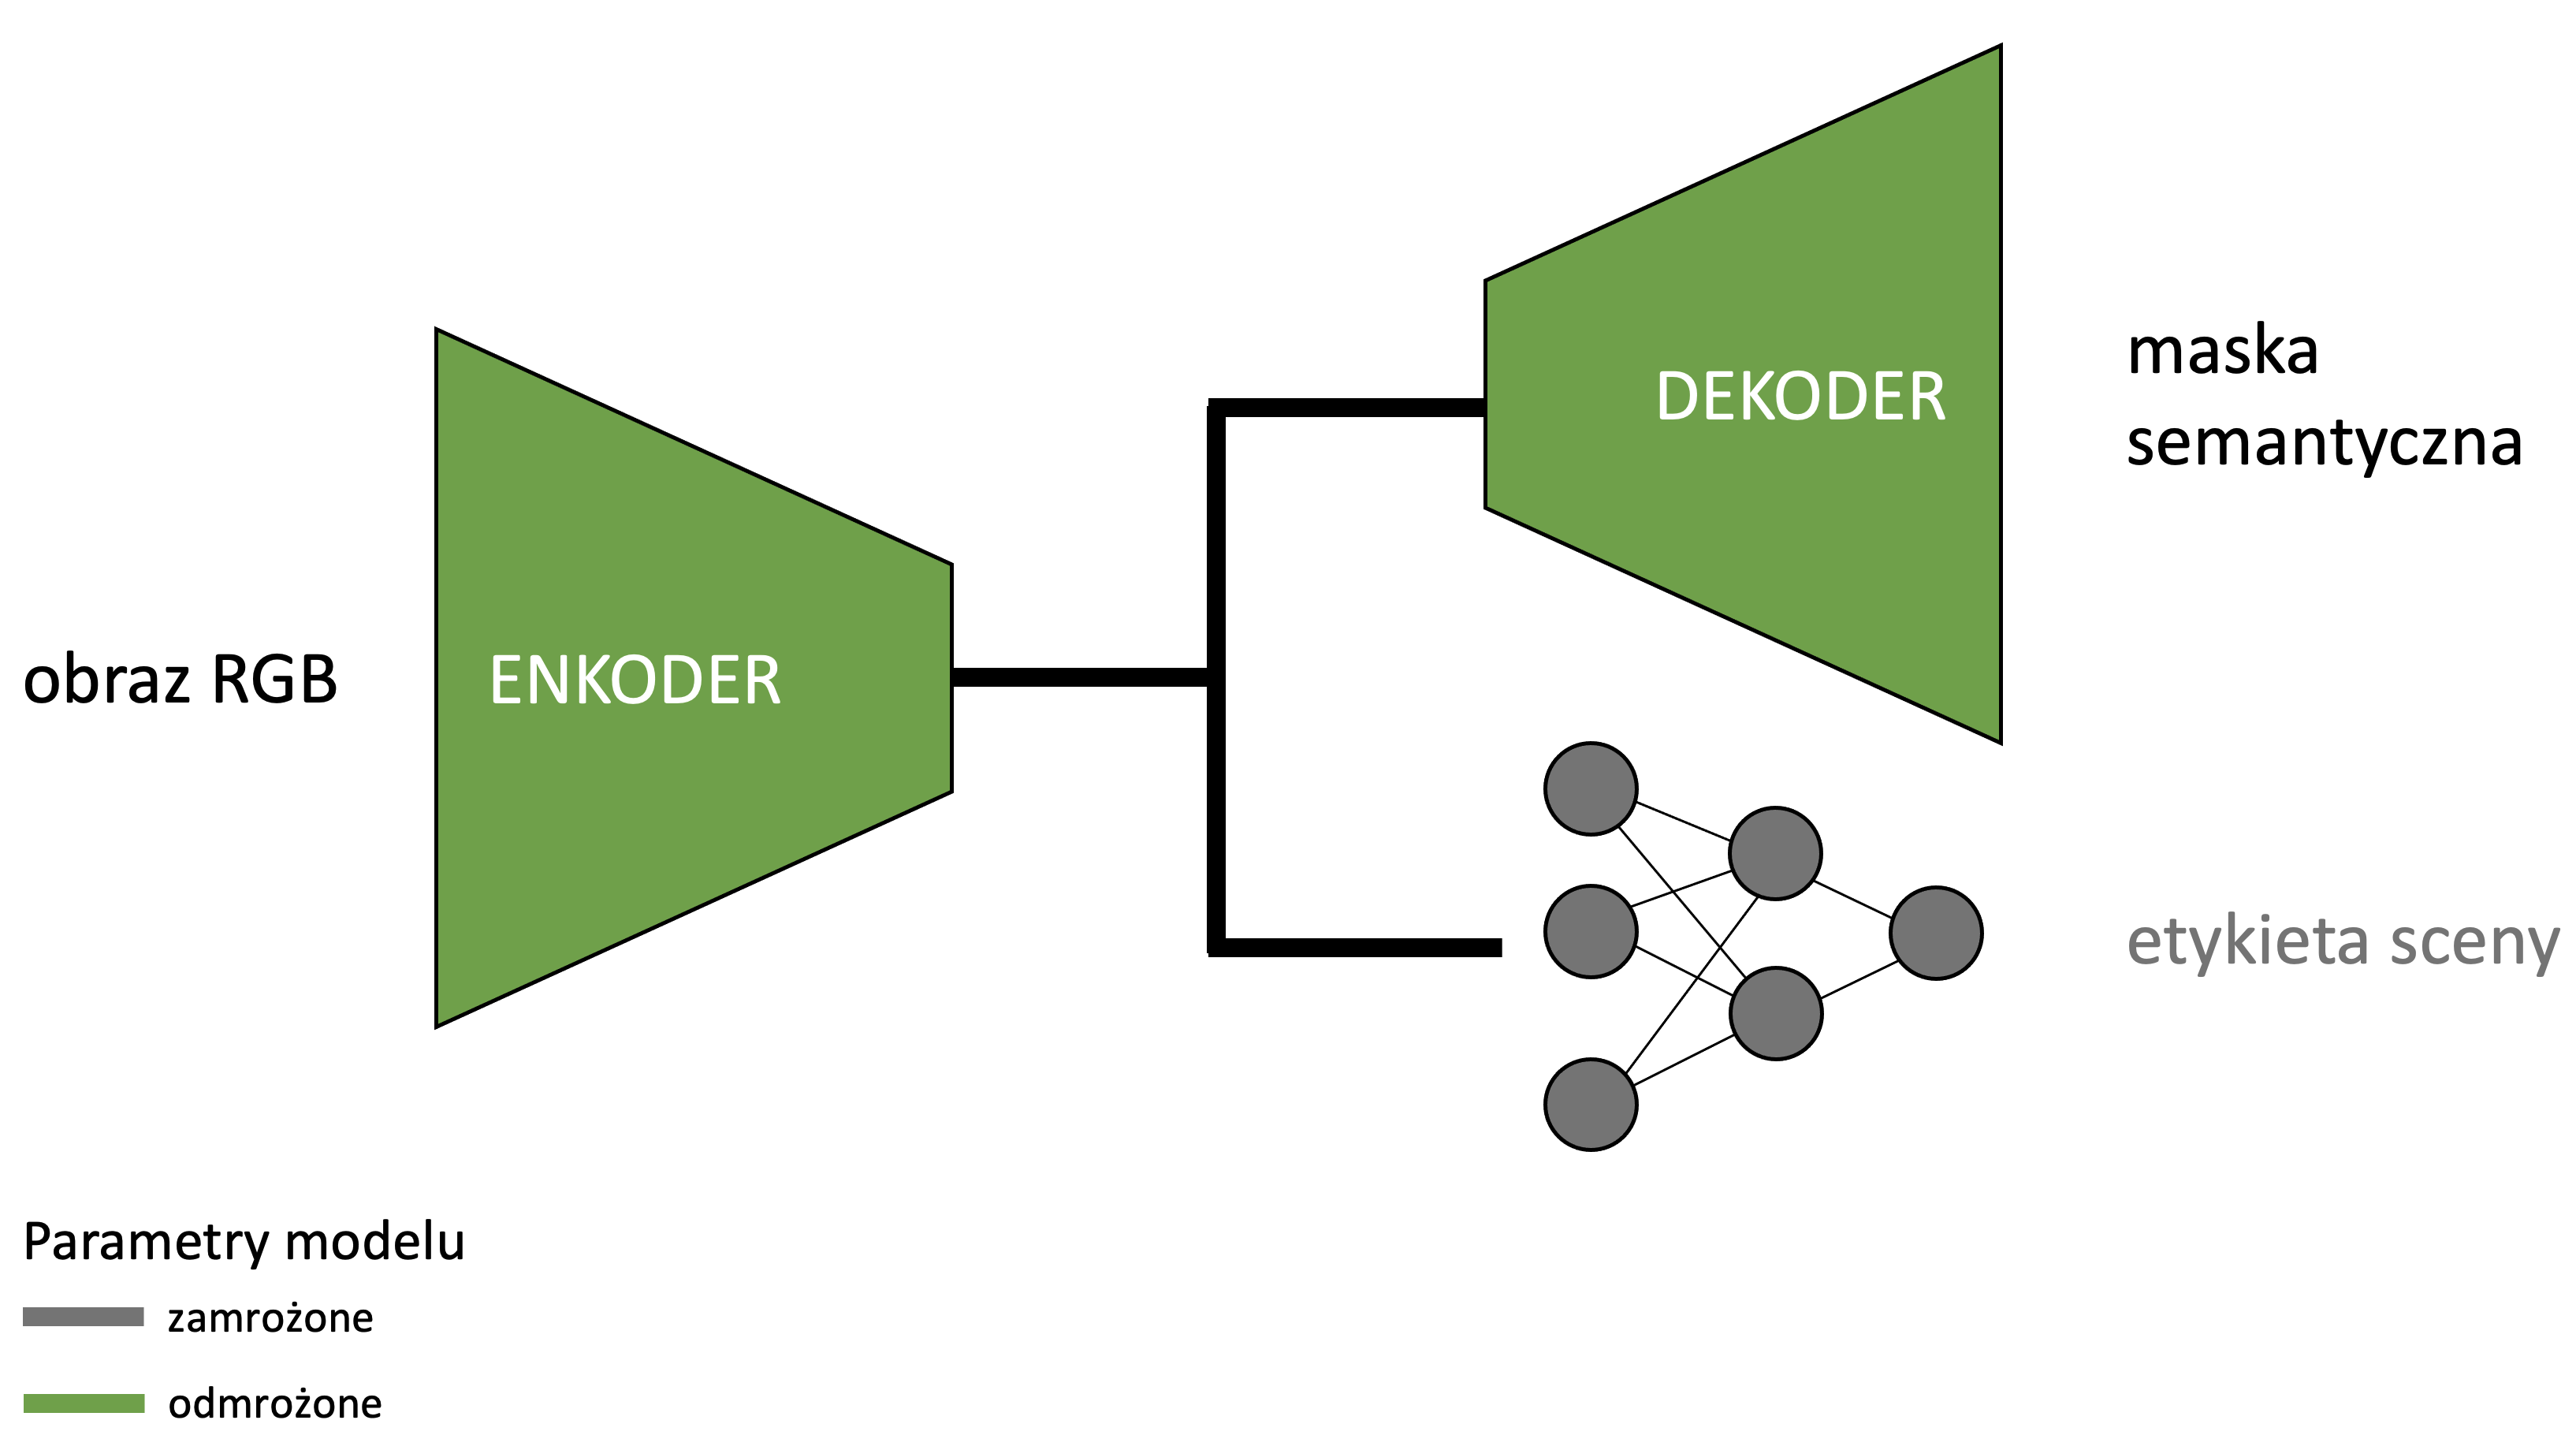
\includegraphics[width=\textwidth]{arch:seg.png}
%         \caption{Architektura sieci wyłącznie w zadaniu segmentacji semantycznej.}
%     \end{subfigure}
%     \caption[]{Podejście jednozadaniowe.}
%     \label{fig:arch-scene-seg}
% \end{figure}

% \begin{figure}[ht!]
%     \centering
%     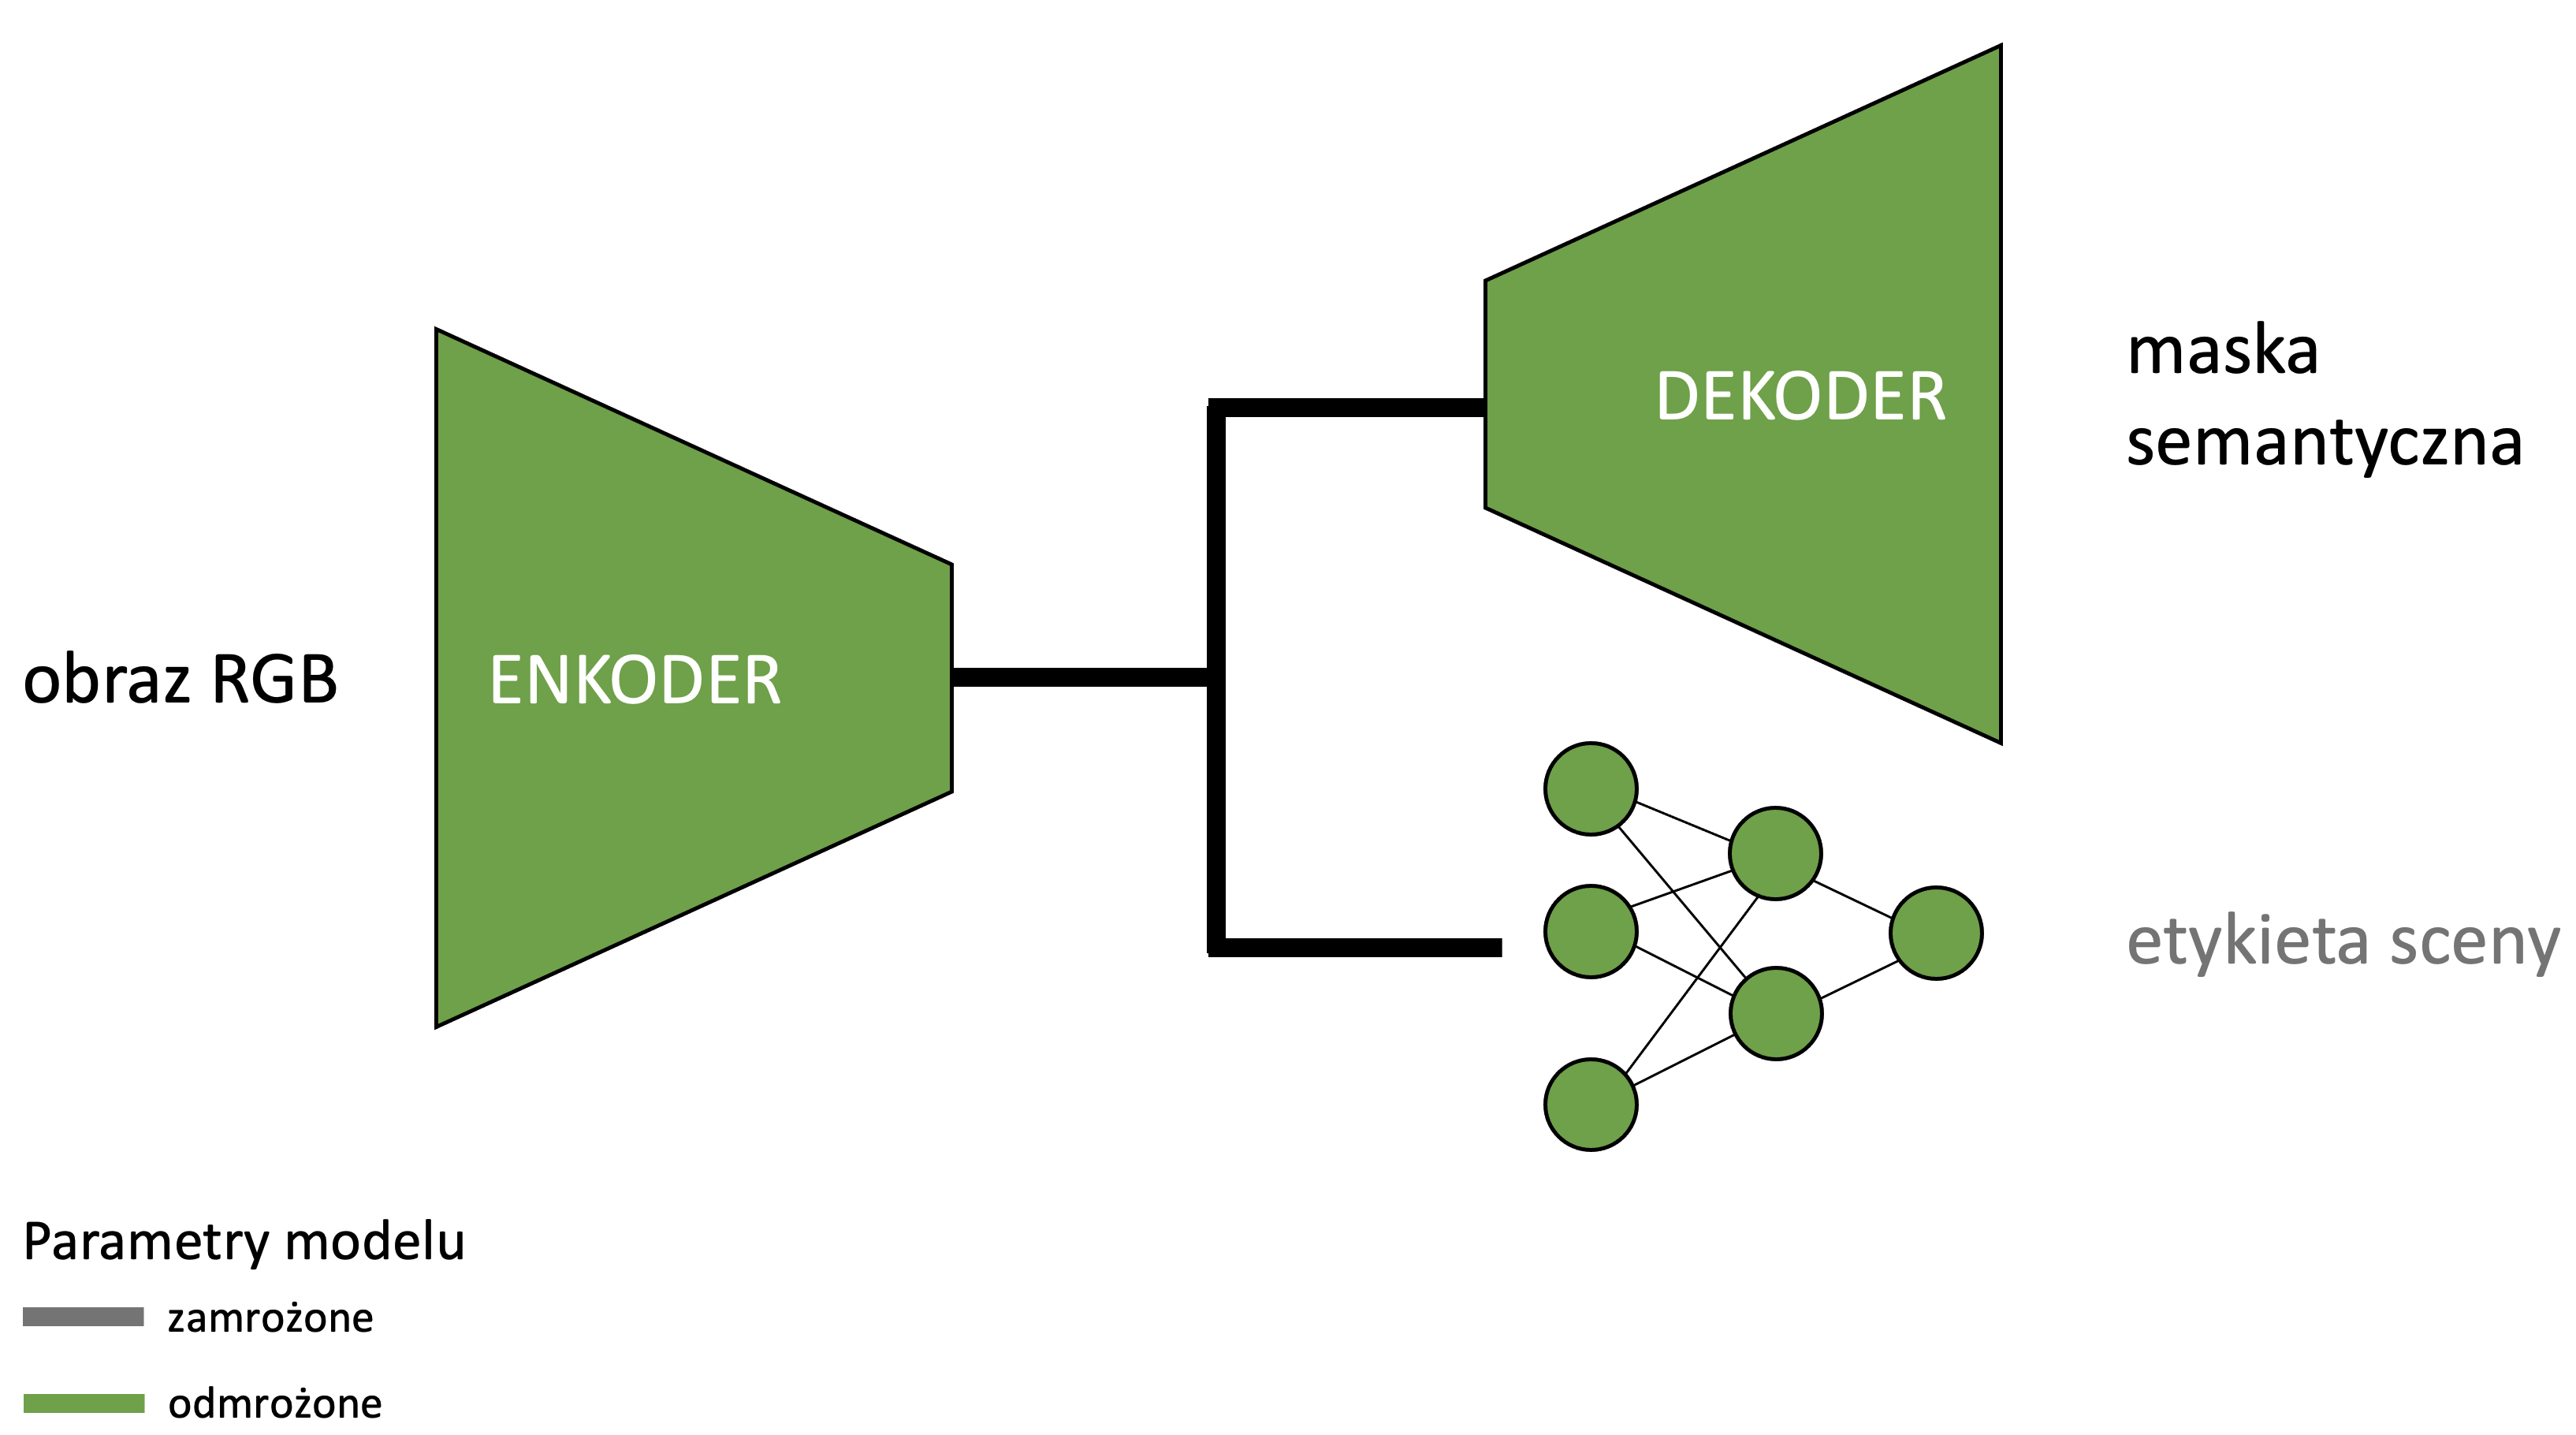
\includegraphics[width=0.75\textwidth]{arch:full.png}
%     \caption{Architektura sieci jako uczenie wielozadaniowego.}
%     \label{fig:arch-full}
% \end{figure}